\documentclass[12pt, twoside]{article}
\usepackage[letterpaper, margin=1in, headsep=0.5in]{geometry}
\usepackage[english]{babel}
\usepackage[utf8]{inputenc}
\usepackage{amsmath}
\usepackage{amsfonts}
\usepackage{amssymb}
\usepackage{tikz}
%\usetikzlibrary{quotes, angles}

\usepackage{graphicx}
\usepackage{enumitem}
\usepackage{multicol}

\usepackage{fancyhdr}
\pagestyle{fancy}
\fancyhf{}
\renewcommand{\headrulewidth}{0pt} % disable the underline of the header

\fancyhead[RE]{\thepage}
\fancyhead[RO]{\thepage \\ Name: \hspace{3cm}}
\fancyhead[L]{BECA / Dr. Huson / 10th Grade Geometry\\* 7 December 2018}

\begin{document}
\subsubsection*{Do Now: Triangle congruence proofs}
 \begin{enumerate}

\item Given $\triangle ABP$ and $\triangle JKP$ with $\angle A \cong \angle J$. $P$ bisects $\overline{AJ}$. Prove $\triangle ABP \cong \triangle JKP$.\\[0.5cm]
  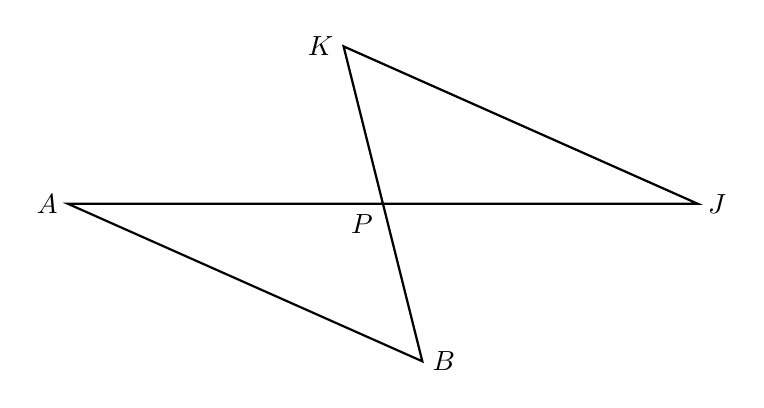
\begin{tikzpicture}
      \draw [thick]
        (0.5,-2)node[right]{$B$}--
        (-0.5,2)node[left]{$K$}--
        (4,0)node[right]{$J$}--
        (0,0)node[below left]{$P$}--
        (-4,0)node[left]{$A$}--cycle;
    \end{tikzpicture}

  \begin{multicols}{2}
    \underline{Statement} \\
    \underline{Reason}
  \end{multicols}
  \begin{multicols}{2}
    \raggedcolumns
    \begin{enumerate}[label={\arabic*)}]
      \item $\triangle ABP$, $\triangle JKP$ \vspace{0.3cm}
      \item \rule{4cm}{0.15mm} \vspace{0.3cm}
      \item \rule{4cm}{0.15mm} \vspace{0.3cm}
      \item $\angle APB \cong \angle JPK$  \vspace{0.3cm}
      \item \rule{4cm}{0.15mm} \vspace{0.3cm}
      \item $\triangle ABP \cong \triangle JKP$ \vspace{0.3cm}
    \end{enumerate}
    \begin{enumerate}[label={\arabic*)}]
      \item Given \vspace{0.3cm}
      \item Given \vspace{0.3cm}
      \item Given \vspace{0.3cm}
      \item \rule{4cm}{0.15mm} \vspace{0.3cm}
      \item Definition of a bisector \vspace{0.3cm}
      \item \rule{4cm}{0.15mm} \vspace{0.3cm}
    \end{enumerate}
  \end{multicols}

  \item Apply the translation $(x,y) \rightarrow (x-1,y+3)$ to the point $A(0,-4)$. \vspace{1cm}
  \item What is the image of $B(4,3)$ under a reflection across the $x$-axis? \vspace{1cm}
  \item State the translation that would map $C(1,5)$ onto $C'(4,3)$. \vspace{1cm}

  \item Express the result to the nearest thousandth.  \vspace{0.5cm}
    \begin{multicols}{2}
      \begin{enumerate}
        \item $\sin 30^\circ = $ \vspace{0.5cm}
        \item $\tan 45^\circ =$
        \item $\sin 28^\circ = $ \vspace{0.5cm}
        \item $\cos 25^\circ =$
      \end{enumerate}
    \end{multicols}

\newpage
  \item Given right $\triangle ABC$ with $AC=12, BC=5, AB=13$, $m\angle C=90^\circ$. Express each trig ratio as a fraction.
    \begin{center}
      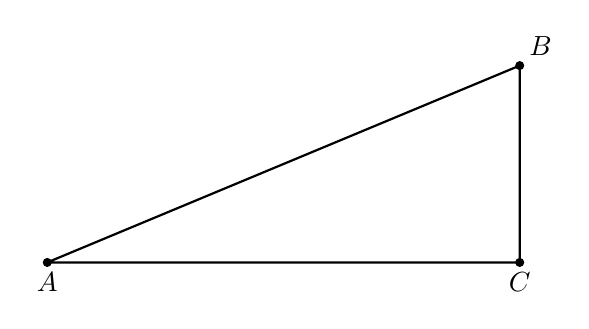
\begin{tikzpicture}[scale=1]
        \draw [thick](0,0)--(6,0)--(6,2.5)--(0,0);
        \draw [fill] (0,0) circle [radius=0.05] node[below]{$A$};
        \draw [fill] (6,0) circle [radius=0.05] node[below]{$C$};
        \draw [fill] (6,2.5) circle [radius=0.05] node[above right]{$B$};
      \end{tikzpicture} \vspace{1cm}
    \end{center}
    \begin{multicols}{2}
      \begin{enumerate}
        \item $\sin A = $ \vspace{1cm}
        \item $\cos A =$
        \item $\sin B = $ \vspace{1cm}
        \item $\tan B =$
      \end{enumerate}
    \end{multicols}

  \item Given right $\triangle ABC$ with $m\angle C=90^\circ$, $m\angle A = 30^\circ$, and $AB=12$.
    \begin{center}
      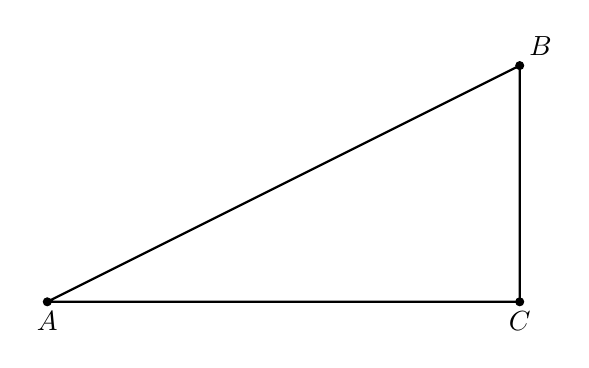
\begin{tikzpicture}%[scale=0.7]
        \draw [thick](0,0)--(6,0)--(6,3)--(0,0);
        \draw [fill] (0,0) circle [radius=0.05] node[below]{$A$};
        \draw [fill] (6,0) circle [radius=0.05] node[below]{$C$};
        \draw [fill] (6,3) circle [radius=0.05] node[above right]{$B$};
      \end{tikzpicture} %\vspace{2cm}
    \end{center}
    \begin{enumerate}
      \item Find $AC$. \vspace{3cm}
      \item Find $BC$. \vspace{3cm}
    \end{enumerate}

\end{enumerate}

\newpage
\setcounter{page}{1}
\subsubsection*{Exit Note: Triangle congruence proof \& transformations assessment}

\begin{enumerate}

\item Given $\triangle QRP$ and $\triangle STP$ with $\overline{QP} \cong \overline{SP}$. $P$ is the midpoint $\overline{RT}$.\\ Prove $\triangle QRP \cong \triangle STP$.\\[0.5cm]
 \begin{tikzpicture}
     \draw [thick]
       (-1,2)node[right]{$R$}--
       (1,-2)node[left]{$T$}--
       (4,0)node[right]{$S$}--
       (0,0)node[below left]{$P$}--
       (-4,0)node[left]{$Q$}--cycle;
   \end{tikzpicture}

 \begin{multicols}{2}
   \underline{Statement} \\
   \underline{Reason}
 \end{multicols}
 \begin{multicols}{2}
   \raggedcolumns
   \begin{enumerate}[label={\arabic*)}]
     \item $\triangle QRP$, $\triangle STP$ \vspace{0.3cm}
     \item \rule{4cm}{0.15mm} \vspace{0.3cm}
     \item \rule{4cm}{0.15mm} \vspace{0.3cm}
     \item $\angle QPR \cong \angle SPT$  \vspace{0.3cm}
     \item \rule{4cm}{0.15mm} \vspace{0.3cm}
     \item $\triangle QRP \cong \triangle STP$ \vspace{0.3cm}
   \end{enumerate}
   \begin{enumerate}[label={\arabic*)}]
     \item Given \vspace{0.3cm}
     \item Given \vspace{0.3cm}
     \item Given \vspace{0.3cm}
     \item \rule{4cm}{0.15mm} \vspace{0.3cm}
     \item Definition of a midpoint \vspace{0.3cm}
     \item \rule{4cm}{0.15mm} \vspace{0.3cm}
   \end{enumerate}
 \end{multicols} \vspace{0.5cm}

 \item Apply the translation $(x,y) \rightarrow (x+1,y+6)$ to the point $A(-5,3)$. \vspace{2cm}
 \item What is the image of $B(2,5)$ under a reflection across the $y$-axis? \vspace{2cm}
 \item State the translation that would map $C(2,-3)$ onto $C'(5,-4)$. \vspace{1cm}


\end{enumerate}

\end{document}
